\section{Future Work}

Our key-value store implementation is far from finished. There are a myriad of ways in which this key-value store can and should be improved upon. We will at least need to implement deletion for both the KVStore module and the B+-Tree module, among some other operations. It would also be good to add durability and support for concurrency. We would also like to extend the B+-Tree cursor concept to create and implement a KVStore Cursor (see Figure \ref{fig:KVStoreCursor1}). 

\begin{figure}[h]
    \centering
    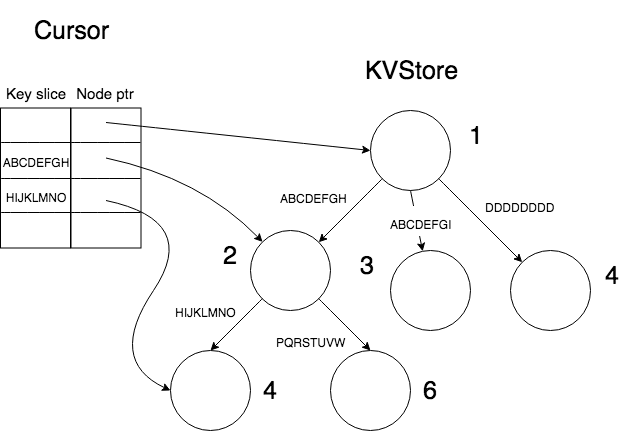
\includegraphics[scale=0.50]{figures/kvcursor1.png}
    \caption{KVStore Cursor at node 4.}
    \label{fig:KVStoreCursor1}
\end{figure}

\begin{figure}[h]
    \centering
    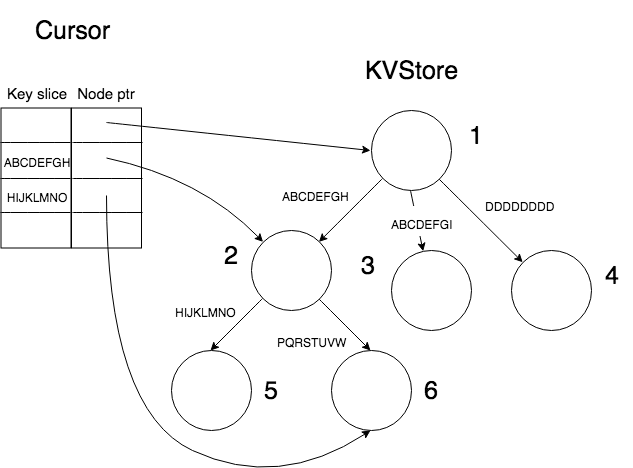
\includegraphics[scale=0.50]{figures/kvcursor2.png}
    \caption{KVStore Cursor at node 6.}
    \label{fig:KVStoreCursor2}
\end{figure}

The KVStore cursor is analogous to the B+-Tree cursor; ancestor nodes in the B+-Tree correspond to ancestor B+-Trees / layers in the KVStore. However, with a KVStore cursor, we would need to also store the key slice that each cursor is located at. This could drastically improve the cost of sequential inserts. This means that when the key of the next operation and the KVStore cursor's current key share a long common prefix, many layers in the KVStore data structure (the trie) will be skipped at the cost of only comparing the search key with the characters associated with each level of the KVStore cursor. We expect this cost to be significantly lower than traversing multiple layers of the overall tree data structure (which also involves navigating through each layer) to get to the desired key. However, it is important to note that if the search keys are totally random, there might be little or not benefit to this scheme. In fact, there would be the added overhead of maintaining KVStore cursor information. 

\begin{comment}
Interesting how in the past sequential i/o was crucial and now this cursor of cursors idea grants great gains when one operates on tree data structures sequentially. 
\end{comment}
